\documentclass[]{article}
\usepackage[utf8]{inputenc}
\usepackage{graphicx}
\usepackage{amsmath}
\usepackage{amsfonts}
\usepackage{amssymb}
\usepackage{subcaption}
%opening
\title{Homework 2}
\author{Ian Hunt-Isaak}
\date{}
\begin{document}

\maketitle


\section{Introduction}
The continuity equation:
\begin{equation}
\frac{\partial}{\partial t} \varphi + \nabla(\varphi \vec{u}) = 0,
\label{eq:continuity}
\end{equation}
with $\varphi$ the value of interest and $\vec{u}$ the velocity field,  is a special case of a conservation equation, in which there are no diffusion or source terms. are those that describe the transport of some physical quantity. This equation describes the flow of an incompressible fluid, such as water, and therefore is a highly useful equation to be able to solve numerically. Unfortunately even something as simple as the continuity equation, Eq. \ref{eq:continuity}, can be incredibly difficult to approach numerically. In simulating this we have the familiar constraint of stability, i.e. that the solution values will not explode, and we also require that our values be positive for all time and space. This latter requirement comes from the fact that when simulating mass transport it would be physically meaningless to have negative matter. 
Without a diffusive term 




In this document we will explore various numerical methods for propagating the Advection - Diffusion - Reaction equation forward in time. This equation describes physical processes and provides an opportunity to explore the limits of stability of numerical methods as well as different approaches to how to propagate time forward. 


\section{Numerical Methods}
In 1-D there are multiple ways to discretize Eq. \ref{eq:
\section{Understanding SHASTA}
The continuous Advection-Diffusion Equation is:



In order to numerically simulate this often physically relevant equation one method is known as the forward Euler method. In this method, space is discretized into a lattice of points with spacing $d$ between them. Likewise, time is discretized with the smallest possible time step being $h$. Using centered differences to replace the full derivatives we can go from a continuous equation to a discrete one:
\begin{equation}
\frac{\varphi^{n+1}_j-\varphi^n_j}{h} = -U \frac{\varphi^n_{j+1}-\varphi^n_{j-1}}{2d} + D \frac{\varphi^n_{j+1}-2\varphi^n_{j}+\varphi^n_{j-1}}{d^2},
\label{eq:discrete_AD1}
\end{equation}
in this equation the superscript represents the time coordinate of $\varphi$ and the subscript, the position on the simulation lattice. Simplifying our notation with $\varphi^n \to \varphi$ and $\varphi^{n+1} \to \hat{\varphi}$, as well as introducing $\alpha = \frac{Uh}{d}$, and $\delta=\frac{Dh}{d^2}$  we can reduce Eq. \ref{eq:discrete_AD1} to:

\begin{equation}
	\hat{\varphi_j} = (\delta+\frac{1}{2}\alpha)\varphi_{j+1} +(1-2\delta)\varphi_{j}+(\delta-\frac{1}{2}\alpha)\varphi_{j-1}. 
	\label{eq:discrete_AD2}
\end{equation}
Giving us a transfer matrix described by $T_{jk} = \{\delta-\frac{\alpha}{2},1-2\delta,\delta+\frac{\alpha}{2}\}$, where the solution could be propagated forward in time by repeatedly multiplying the matrix T with the vector of point values $\vec{\varphi}$. 
This is a result that would could have immediately arrived at if we considered the following relation of spatial derivatives to the transfer matrix.
\begin{equation}
\frac{d}{dx} \Leftrightarrow \frac{1}{2d}\{-1,0,1\},
\label{eq:dx}
\end{equation}
\begin{equation}
\frac{d^2}{dx^2} \Leftrightarrow \frac{1}{d^2}\{1,-2,1\}
\label{eq:dx^2}
\end{equation}
%

\begin{equation}
T_{ADR}=\begin{bmatrix} 
1       & 0 & 0 &\dots& \dots &0&0 \\
a      & c & b & 0&\dots & 0 &0\\
0& a & c & b & 0 &\dots & 0 \\
\hdotsfor{7} \\
0 &\dots & \dots & 0&a & c & b  \\
0     &0  & 0 & \dots&\dots & 0&1
\end{bmatrix}
\label{eq:T_Diffusion_2}
\end{equation}
where $a = \delta +\frac{\alpha}{2}$, $b =\delta-\frac{\alpha}{2}$, and $c=1-2\delta +\kappa$, with $\kappa = r h$. 


\begin{figure}
	\begin{subfigure}{.5\textwidth}
		\centering
		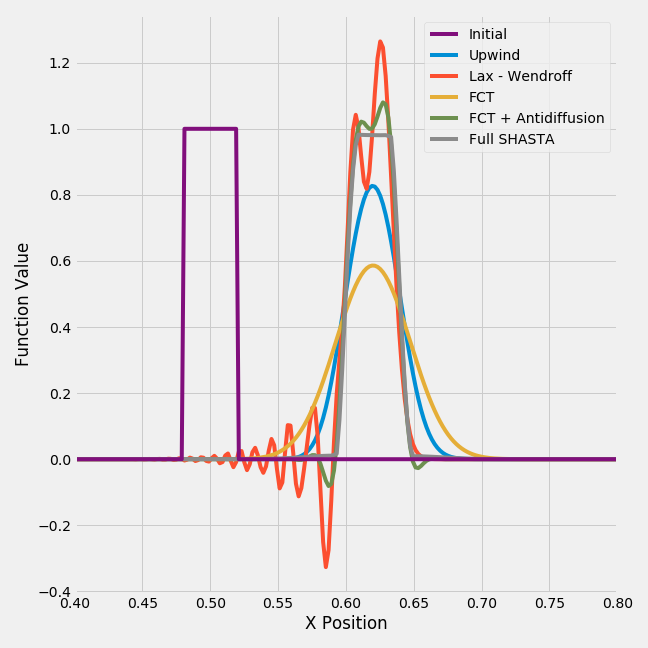
\includegraphics[width=.8\linewidth]{figures/constU_fCompare.png}
		\caption{}
	\end{subfigure}%
	\begin{subfigure}{.5\textwidth}
		\centering
		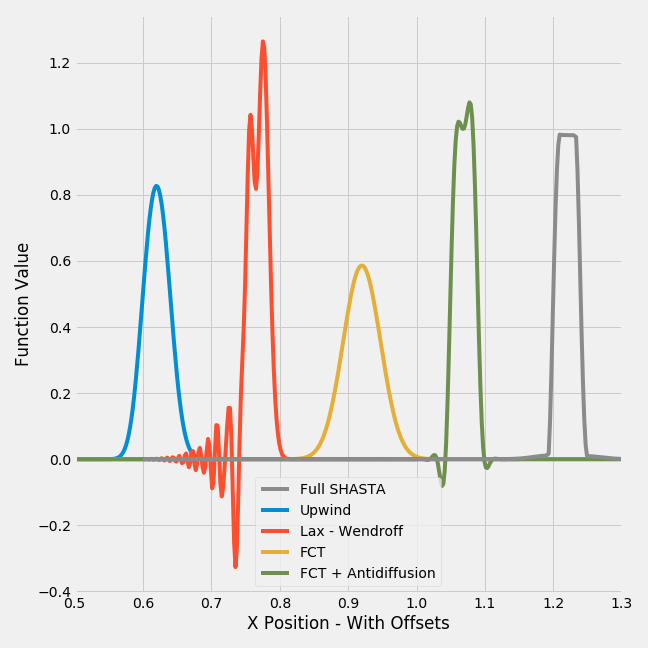
\includegraphics[width=.8\linewidth]{figures/constU_fCompare_offset.png}
		\caption{}
	\end{subfigure}
	\caption{}
	\label{fig:constU_f_compare}
\end{figure}
\begin{figure}

		\centering
		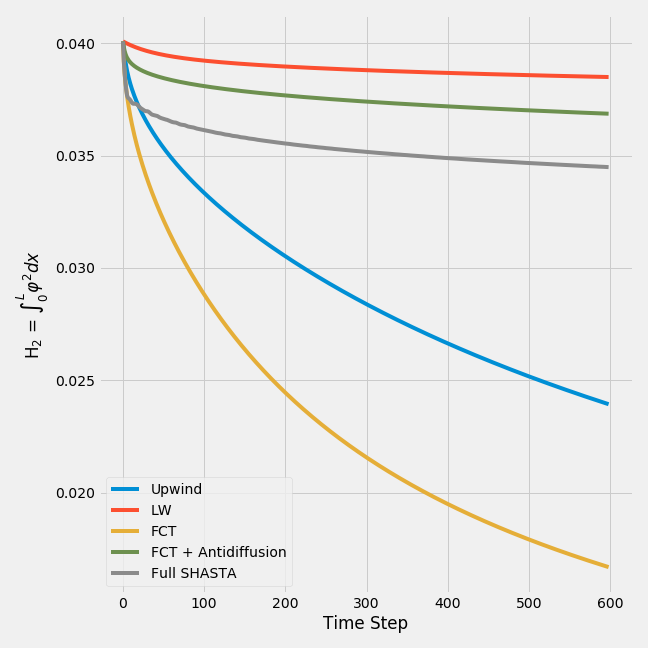
\includegraphics[width=.8\linewidth]{figures/constU_compareH.png}
		\caption{}
	\label{fig:constU_compareH}
\end{figure}

  \begin{thebibliography}{1}
  	
  	\bibitem{shasta} Boris, J. P. \& Book, D. L. Flux-corrected transport. I. SHASTA, a fluid transport algorithm that works. Journal of computational physics 11, 38–69 (1973).
  	

  \end{thebibliography}



\end{document}
